\documentclass[conference]{IEEEtran}

% Document properties
\title{On-chip order-exploiting routing table minimization for a multicast supercomputer network}
\author{%
  \IEEEauthorblockN{Andrew~Mundy, Jonathan~Heathcote and Jim~D.~Garside}
  \IEEEauthorblockA{School of Computer Science,\\
                    University of Manchester, UK}
}

% Prettier tables
\usepackage{booktabs}

% Pictures
\usepackage{graphicx}

% Diagrams
\usepackage{tikz}
\usepackage{ifthen}
\usetikzlibrary{ calc
               , backgrounds
               , positioning
               , decorations.pathreplacing
               , decorations.markings
               , arrows
               , positioning
               , automata
               , shadows
               , fit
               , shapes
               , arrows
               , patterns
               , spy
               }

% Pseudo-code
\usepackage{clrscode3e}

% Force float positions in some cases
\usepackage{float}

% Better math environments
\usepackage{amsmath}

% Neaten the fixed-width font
\usepackage{sourcecodepro}
\newcommand{\mytt}[1]{\texttt{\footnotesize#1}}

\usepackage[binary-units]{siunitx}
\usepackage[caption=false, font=footnotesize]{subfig}

%% Bibliographies
\usepackage[backend=bibtex, style=ieee, doi=false, url=false, mincitenames=1, maxcitenames=2, maxbibnames=7]{biblatex}
\renewcommand*{\bibfont}{\small}
\bibliography{paper}

\begin{document}
  \maketitle

  \begin{abstract}
SpiNNaker is a many-core supercomputer, designed for the simulation of large neural-networks; cores communicate with multicast packets.
Routing within SpiNNaker is controlled by ternary content addressable memories (TCAM) of quite limited size.
However, not all neural-network applications will result in routing tables sufficiently small to fit in TCAM and some minimization is necessary.
In this paper we argue that existing minimization techniques either do not result in sufficiently minimized tables or cannot be implemented within the small code and memory footprint available to a SpiNNaker core.
To resolve these issues we present a new algorithm which exploits the ordered nature of the TCAM to achieve good compression of routing tables while meeting the code-space and memory constraints of the SpiNNaker platform.

  \end{abstract}

  \section{Introduction}

SpiNNaker~\parencite{Furber2014} is a purpose-built supercomputer intended to facilitate the simulation of large biological neural networks.
Software models are distributed across a network of processors which communicate by passing (short) messages.
Neurons in the brain typically have a `fanout' of the order of thousands \parencite{TODO} and SpiNNaker's interconnection structure reflects this in that it supports multicasting network packets to an arbitrary set of destinations.

Each SpiNNaker chip has a single router capable of steering packets to or from the 18~on-chip processor cores and inter-chip links.
The inter-chip network is a triangularly connected 2D surface, which may be wrapped into a torus to provide greater aggregate bandwidth.
This can be drawn as a hexagonal mesh but is sometimes more conveniently pictured skewed into squares.
The six inter-chip links are typically labelled with compass points (\figurename~\ref{fig:diagrams/topology}).

\begin{figure}[!b]
  
  \center
  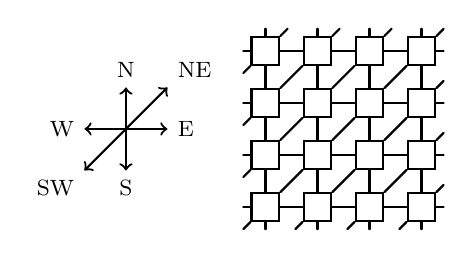
\begin{tikzpicture}[thick, font=\footnotesize, line cap=round]
	
	\pgfmathtruncatemacro{\width}{4}
	\pgfmathtruncatemacro{\height}{4}
	
	\pgfmathsetlengthmacro{\sep}{0.8em}
	\pgfmathsetlengthmacro{\size}{1em}
	
	\pgfmathsetlengthmacro{\compass}{1.5em}
	
	% Draw (and label) a chip
	% #1: x
	% #2: y
	% #3: extra options
	\newcommand{\chip}[3]{
		\node (x#1y#2)
		      [ minimum width=\size
		      , minimum height=\size
		      , node distance=\sep
		      , inner sep=0
		      , draw
		      , #3
		      ]
		      {};
	}
	
	% Draw the chips
	\chip{1}{1}{}
	\foreach [count=\lasty] \y in {2,...,\height}{
		\chip{1}{\y}{above=of x1y\lasty}
	}
	\foreach \y in {1,...,\height}{
		\foreach [count=\lastx] \x in {2,...,\width}{
			\chip{\x}{\y}{right=of x\lastx y\y}
		}
	}
	
	% Draw NE/SW Links
	\foreach [count=\lastx] \x in {2,...,\width}{
		\foreach [count=\lasty] \y in {2,...,\height}{
			% NE/SW
			\draw (x\lastx y\lasty) -- (x\x y\y);
		}
	}
	
	% Draw N/S Links
	\foreach  \x in {1,...,\width}{
		\foreach [count=\lasty] \y in {2,...,\height}{
			% NE/SW
			\draw (x\x y\lasty) -- (x\x y\y);
		}
	}
	
	% Draw E/W Links
	\foreach [count=\lastx] \x in {2,...,\width}{
		\foreach \y in {1,...,\height}{
			% NE/SW
			\draw (x\lastx y\y) -- (x\x y\y);
		}
	}
	
	% Draw outer links along top and bottom
	\foreach \x in {1,...,\width}{
		% NE/SW
		\draw (x\x y\height) -- +(+\sep, +\sep);
		\draw (x\x y1) -- +(-\sep, -\sep);
		
		% N/S
		\draw (x\x y\height) -- +(0, +\sep);
		\draw (x\x y1) -- +(0, -\sep);
	}
	
	% Draw outer links along left and right
	\foreach \y in {1,...,\height}{
		% NE/SW (NB: prevent redrawing of corner diagonals)
		\ifthenelse{\y < \height}{
			\draw (x\width y\y) -- +(+\sep, +\sep);
		}{}
		\ifthenelse{\y > 1}{
			\draw (x1y\y) -- +(-\sep, -\sep);
		}{}
		
		% E/W
		\draw (x\width y\y) -- +(+\sep, 0);
		\draw (x1y\y) -- +(-\sep, 0);
	}
	
	
	% Draw the 'compass'
	\coordinate (center) at ([xshift=-3.0*\compass]$(x1y1.west)!0.5!(x1y\height.west)$);
	
	\draw [->] (center) -- ++(\compass, \compass) node [anchor=south west] {NE};
	\draw [->] (center) -- ++(-\compass, -\compass) node [anchor=north east] {SW};
	\draw [->] (center) -- ++(\compass, 0) node [anchor=west] {E};
	\draw [->] (center) -- ++(-\compass, 0) node [anchor=east] {W};
	\draw [->] (center) -- ++(0, \compass) node [anchor=south] {N};
	\draw [->] (center) -- ++(0, -\compass) node [anchor=north] {S};
	
\end{tikzpicture}


  
  \caption{SpiNNaker chips (squares) in a triangular torus topology. Wrap-around links omitted for clarity.}
  \label{fig:diagrams/topology}
  
\end{figure}

Packets are routed around this network by Address Event Representation (AER)~\parencite{Boahen2000}; each packet contains a routing key which identifies its source and routers forward (and may duplicate) packets towards their destination(s).
SpiNNaker uses 32-bit routing keys, which reflect the intended scale of the system.
Packets are recognised using a Ternary Content Addressable Memory (TCAM) which bit-masks keys before looking for particular matches,
this means that each key bit can be matched with binary \mytt{0}, \mytt{1}, or \mytt{X} (`don't care').
In addition the TCAM is prioritised such that only the first-found match will be returned, allowing `catch all' entries to be inserted near the bottom of the table.
Finally, if a key is not found in the table, the packet is `default routed' continuing in the direction it arrived (e.g., an unrecognised packet arriving via the East link is default routed out of the West link).

For example, given a simplified routing table with 4-bit keys

\begin{table}[H]
  \centering
  \begin{tabular}{c l}
    \toprule
    Key-Mask & Route \\
    \midrule
    \texttt{0000} & \texttt{NE N}\\
    \texttt{X111} & \texttt{S}\\
    \texttt{1XXX} & \texttt{3 4}\\
    \bottomrule
  \end{tabular}
\end{table}

\noindent any packets with the keys \mytt{0111} or \mytt{1111} would match the second entry in the table and be routed out of the South link.
Packets with the key \mytt{0000} would instead match only the first entry and would be routed out of both the North East and North links.
Other packets beginning with a \mytt{1} would match the last entry and be routed to the indicated processing cores.
All other packets would be unrecognised by the router and be default routed in a straight line, e.g., a packet arriving on the South West link with the key \mytt{0011} would be routed out of the North East link.

The TCAM was chosen with an arbitrary size of \num{1024}~entries, believed large enough for most applications although making entries quite precious.
Indeed, it is not always possible to avoid exceeding this limit on routing table size -- particularly for neural networks which feature large `fanin' or `fanout' routes.
As the largest SpiNNaker machine will consist of \num{57600}~chips, and the same number of TCAM routing tables, it is desirable to exploit the massive parallelism of SpiNNaker to perform any minimisation of routing tables rather than to minimise tables externally before loading them to the machine. As we will show, this presents a challenge due to the limited on-chip memory available.

\section{Routing table minimization}

To indicate the importance of routing table minimization to SpiNNaker we constructed two benchmark networks.
In the first of these networks each processing core in a 144-chip system is connected to every other core in the system with a probability determined by the distance between the cores.
In our model the probability of there being a connection between two cores is given by $\frac{1}{2}\exp(-0.65d)$ where $d$ is the number of hops in the shortest path between the cores.
This benchmark models networks in which processing cores are strongly connected to their neighbours but are weakly connected to distant chips \textbf{EXAMPLE AND REFERENCE}.

The second benchmark extends the first benchmark by adding a number of longer distance connections to the network and is based on the `centroid' model of \textcite{Navaridas2015}.
In this model a small number of cores are connected to a group of cores located at some distance across the machine.
Each core has a \SI{10}{\percent} chance of being connected to a single, distant, group of cores and a \SI{5}{\percent} chance of being connected to two distant groups.
\figurename~\ref{fig:experiment/setup} illustrates these two benchmarks and shows the probability of a single core being connected to other cores within the network.

\begin{figure}
  \centering
  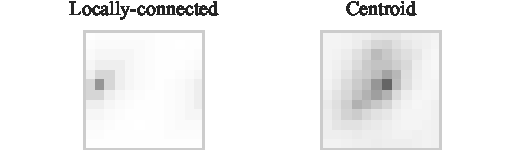
\includegraphics{experiments/experiments.pdf}
  \caption{Map of the probability of a single core being connected to cores on surrounding chips for the two benchmarks. Darker means higher probability.
           In the above centroid model the core is connected to two clusters of cores (toward the south west and north west).}
  \label{fig:experiment/setup}
\end{figure}

Once the connectivity of the benchmarks was determined, the Neighbour Exploring Routing (NER) algorithm~\parencite{Navaridas2015} was used to generate the routes taken by packets across the network.
While this algorithm has been shown to effectively exploit `default routing' to reduce the size of routing tables the resulting routing tables, of both our benchmarks, were too large to fit in the number of entries available (see \figurename~\ref{fig:results/final}).

Routing keys were assigned such that packets originating on the $p$th core of the chip at $(x, y)$ in the skewed mesh used the two most significant bytes in the 32-bit key to represent the $x$ and $y$ co-ordinates and the following five bits to indicate the core ID, $p$.
The remaining 11 bits of the key were left blank, i.e.,~\mytt{X} in the routing tables.
This key assignation scheme, \textit{XYP}, is common in SpiNNaker applications~\parencite{Davies2012}.

\textcite{Liu2002} presented a method for using Espresso-II~\parencite{Brayton1984} to minimize routing tables for IP routers.
In this method a routing table is partitioned in subtables in which entries have equivalent routing destinations and prefix length.
Each subtable is minimized using Espresso to produce a functionally equivalent but smaller set of entries.
\figurename~\ref{fig:results/final} shows the result of applying this technique to the routing tables from our benchmarks once entries which could be replaced by default routing were removed.
In the case of the `locally-connected' benchmark a combination of default routing and logic minimization is able to reduce the majority, but not all, of the 144 routing tables to fewer than \num{1024}~entries.
In the more challenging centroid model this technique is unable to reduce any tables to fit within the TCAM constraint.

In contrast to the unicast IP routing tables at which minimization is normally targeted SpiNNaker routing tables are multicast.
Consequently, there are two factors which may explain the poor compression ratios achieved by the above technique when applied to SpiNNaker routing tables.
Firstly, while the IP routing tables discussed by \textcite{Liu2002} have relatively few output ports, each SpiNNaker router has the equivalent of up to $2^{24}$ unique routes -- consequently the number of entries with equivalent routes can be expected to be much smaller.
Secondly, whereas IP addresses are assigned such that very coarse routing decisions may be made from very few bits, multicasting potentially reduces the amount of mutual information between keys which describe similar routes since keys are related to route origins not destinations.

\subsection*{``Order-exploiting'' minimization}

Unlike IP routing tables, SpiNNaker routing tables can be expected to be largely static.
As such, logic minimization which does not preserve exact equivalence, but instead matches a superset of the routing keys used, may be used to generate routing tables with far fewer entries.
For example, the first two entries in the table

  \begin{table}[H]
    \centering
    \begin{tabular}{c l l}
      \toprule
      Key-Mask & Route \\
      \midrule
      \texttt{0001} & \texttt{N} \\
      \texttt{0010} & \texttt{N} \\
      \texttt{1111} & \texttt{S} \\
      \bottomrule
    \end{tabular}
  \end{table}

\noindent may be combined into a new entry (\mytt{00XX}) which would match more keys than were matched by the original two entries.
In IP routing tables, which are considerably larger than those in SpiNNaker and are highly dynamic, this minimization would be avoided as it would (a) require the minimizer to inspect the entire table during minimization to avoid breaking the functionality of the table,
and (b) slow down the process of updating the table to deal with changed routes.
However, in the case of SpiNNaker -- and other systems with largely static routing tables and very tight constraints on entries -- this technique can allow for significant reductions in table size.

We extended the technique of \textcite{Liu2002} to investigate the effect of this on our benchmark networks.
First, each routing table was split into subtables of entries with the same route.
Next the subtables were sorted such that subtables with fewer entries were moved to the top of the routing table and larger ones toward the bottom.
Finally, the minimization procedure from Espresso was applied to each subtable in turn.
However, unlike the technique proposed by \textcite{Liu2002}, we allowed Espresso to generate entries which matched a superset of keys matched by the original entry provided that they did not match keys expected to match entries in lower subtables.
The minimized table depends on TCAM ordering to ensure that it is functionally equivalent to the original.
We call this use of table ordering to achieve greater compression of entries ``order-exploiting'' minimization.

\figurename~\ref{fig:results/final} shows that this new technique for reducing routing table size is sufficient to minimize all the routing tables in our benchmarks to fit within the 1024-entry size required by SpiNNaker.

\subsection*{On-chip logic minimization}

Espresso is capable of rapidly minimizing routing tables of the scale shown in our benchmarks, for example \textbf{TIMING FOR SINGLE TABLE}.
However, as projected SpiNNaker machines are expected to consist of nearly sixty-thousand chips, and the same number of routing tables, the  compute time required to minimize all tables is likely to be significant, \textbf{FOR EXAMPLE SEVERAL HOURS}.
Minimization on this scale is an `embarrassingly'-parallel problem, and the wall-clock time required to perform this task for SpiNNaker may be significantly reduced by performing the minimization directly on the chips to which the routing tables relate.

Processing cores in SpiNNaker have access to \SI{64}{\kibi\byte} of data tightly-coupled memory (DTCM) and \SI{32}{\kibi\byte} of instruction tightly-coupled memory (ITCM).
This places severe limitations on the programs which they may execute.
While we have shown that Espresso may be used to perform order-exploiting minimization for use with SpiNNaker, its memory usage and code size preclude its use on embedded systems~\parencite{Lysecky2003}.
In contrast, m-Trie minimization~\parencite{Ahmad2007} has been shown to be capable of effectively compressing IP routing tables while consuming very little memory (as low as \SI{16}{\kibi\byte}) but is not suitable for use when order-exploiting minimization is required (see \figurename~\ref{fig:results/final}).

\section{Ordered-Covering}

  We present a novel algorithm called ``Ordered-Covering'' which is capable of performing order-exploiting routing table minimization within the small memory and code-space available on SpiNNaker.
  The algorithm proceeds by sequentially \textit{merging} sets of routing table entries with the same output routes while ensuring these merged entries do not \textit{cover} existing entries. 
  A set of routing entries is merged by replacing them with one new entry containing only the bits common to all the original entries and \mytt{X}s for all other bits
  (e.g., \mytt{1010} and \mytt{0110} would be merged to produce \mytt{XX10}).
  A routing entry covers another when the set of keys matched by one entry intersects with those of another below it in the table.

  In addition, we annotate each entry in the table with the set of keys that it is expected to match, the \textit{aliases} of the entry.
  An empty aliases set simply means that the entry is expected to match all of the packets which would be matched by its key.
  For example, merging the first two entries in the following table would generate a new entry with the original keys listed as aliases:

  \begin{figure}[H]
    \centering
    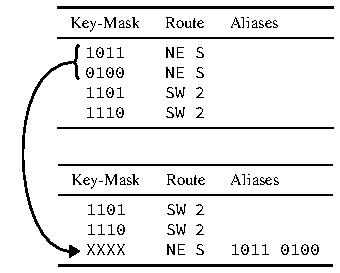
\includegraphics{figures/aliases_example}
  \end{figure}

  \begin{figure*}
    \subfloat[%
      A merge which does not obey the \textit{up-check} rule~(2a).
      Before the merge a packet with key \mytt{0011} would have been routed to \mytt{E~S}; after the merge the same packet would be routed to \mytt{N} instead.
      This is because the merge has resulted in the correct entry being moved below an entry which \textit{covers} it.
    ]{%
      \label{fig:algorithm/rule2a_example}
      \begin{minipage}{.95\columnwidth}
        \centering
        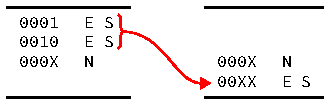
\includegraphics{figures/rule2a_example}
      \end{minipage}
    }
    \hfill
    \subfloat[%
      A merge which does not obey the \textit{down-check} rule~(2b).
      Before the merge a packet with key \mytt{1100} would have been routed to \mytt{NE~S}; after the merge the same packet would be routed to \mytt{SW 2} instead.
      This is because the merge has resulted in the insertion of a new entry which \textit{covers} an existing entry.
    ]{%
      \label{fig:algorithm/rule2b_example}
      \begin{minipage}{.95\columnwidth}
        \centering
        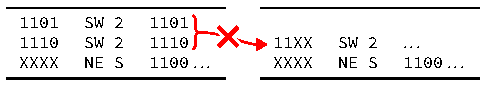
\includegraphics{figures/rule2b_example}
      \end{minipage}
    }
    \caption{Examples of invalid merges as defined by the \textit{Ordered-Covering} rules}
    \label{fig:algorithm/rules}
  \end{figure*}

  When minimizing a routing table, the following \textit{Ordered-Covering rules} are used:

  \begin{enumerate}[\IEEEsetlabelwidth{3)}]
    \item Routing tables must be ordered as follows:
      \begin{enumerate}[\IEEEsetlabelwidth{a)}]
        \item Firstly, in increasing order of \textit{generality}, i.e., the number \mytt{X}s contained in their keys and masks.
              For example, an entry with the key-mask of \mytt{00XX} (\textit{generality} of 2) must be placed below any entries with fewer \mytt{X}s in their key-masks, e.g., below \mytt{0000} and \mytt{00X1} (generalities of 0 and 1 respectively).
        \item Secondly, new entries must be inserted below existing entries of equivalent generality.
              For example, if \mytt{XX00} were already present in the table the new entry \mytt{0XX1} must be inserted below it.
      \end{enumerate}
    \item The only merges allowed are those which would not:
      \begin{enumerate}[\IEEEsetlabelwidth{b)}]
        \item cause any entry in the merge to become \textit{covered} by an entry higher up the table.
              This rule is referred to as the \textit{up-check} rule.
              A merge that would be disallowed by this rule is shown in \figurename~\ref{fig:algorithm/rules}\subref{fig:algorithm/rule2a_example}.
            \item cause any entry or \textit{aliased entry} below the merge to become \textit{covered}, see \figurename~\ref{fig:algorithm/rules}\subref{fig:algorithm/rule2b_example}.
              This rule is referred to as the \textit{down-check} rule.
      \end{enumerate}
  \end{enumerate}

  A simple, greedy, algorithm to minimize a routing table according to these rules is:\par\nopagebreak
  \begin{codebox}
    \Procname{$\proc{Minimize}(\id{table}, \id{target})$}
    \li \While $\attrib{table}{length} >  \id{target}$
    \li \Do $\id{merge} \gets \proc{Get-Largest-Merge}(\id{table})$
    \li     \If $\attrib{merge}{isEmpty}$
    \li     \Then \kw{break} \End
    \li     $\id{table} \gets \proc{Apply-Merge}(\id{table}, \id{merge})$
        \End
    \li \Return $\id{table}$
  \end{codebox}

  \noindent Where:
  \begin{itemize}
    \item $\id{table}$ is a routing table that is sorted according to rule~(1)
    \item $\proc{Get-Largest-Merge}$ is a function which returns a (possibly empty) set of routing table entries which may be merged without breaking the up- or down-check rules~(2)
    \item $\proc{Apply-Merge}$ merges the set of routing entries and uses rule~(1) to determine where the new entry should be inserted into the table
  \end{itemize}

  The algorithm terminates early if $\attrib{table}{length} \le \id{target}$ which can save a large amount of time in comparison to fully minimizing the table.

  The $\proc{Get-Largest-Merge}$ function is where the algorithm spends most of its time and we present one possible implementation in the remainder of this section.
  Our implementation considers merging all groups of entries in the table which share the same set of output ports.
  In practice, merging these groups will often violate either rule~(2a)~or~(2b).
  Rather than immediately rejecting these merge candidates, we use a pair of simple greedy approaches to iteratively remove entries from merge candidates until both rules are obeyed.
  We split our approach into two phases, the first refines merge candidates until they obey the up-check rule and the second does the same for the down-check rule.

  \subsection{Resolving the up-check}

  For each merge candidate we inspect every entry in the merge to ensure it does not break the up-check rule~(2a).
  When inspecting an entry, $e$, in the merge candidate we scan through the entries between $e$ and the position where the merged entry would be inserted.
  If any entry is found which would cover $e$, $e$ is removed from the merge candidate and we proceed to check the next entry in the candidate merge.

  For example, consider the table:\par\nopagebreak
  \begin{figure}[H]
    \centering
    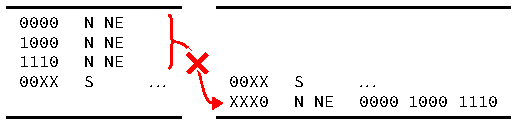
\includegraphics{figures/upcheck_resolve_example_1}
  \end{figure}

  \noindent Initially we could consider merging the first three entries.
  Doing so would mean that \mytt{0000} would be combined into the new entry \mytt{XXX0}, positioned below \mytt{00XX}.
  However, \mytt{00XX} would cover then \mytt{0000}.
  As moving \mytt{0000} below \mytt{00XX} by including it in the merge would change the behaviour of the routing table, \mytt{0000} may not be included in the merge.
  After removing \mytt{0000} the, refined, merge is:\par\nopagebreak
  \begin{figure}[H]
    \centering
    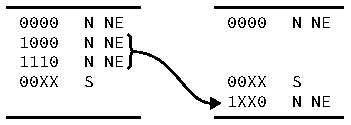
\includegraphics{figures/upcheck_resolve_example_2}
  \end{figure}

  \noindent Since the remaining entries in the merge candidate (\mytt{1000} and \mytt{1110}) are not covered by \mytt{00XX} (the only entry between their current positions and the location where the merge is inserted), the refined merge obeys the up-check rule.

  \subsection{Resolving the down-check}

  The \textit{up-check} ensures that an entry, $e$, cannot -- through being merged with other entries -- become covered by being moved below another entry which matches a subset of the keys matched by $e$.
  The \textit{down-check} instead ensures that the entry resulting from a merge would not match a subset of the packets expected to match entries below the point where the entry resulting from the merge would be located.
  
  For example, consider the table:\par\nopagebreak
  \begin{figure}[H]
    \centering
    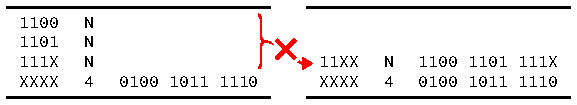
\includegraphics{figures/downcheck_resolve_example_1}
  \end{figure}

  \noindent Our initial merge candidate, the first three entries, would result in the insertion of the entry \mytt{11XX} immediately above the bottom entry.
  However, \mytt{11XX} matches \mytt{1110}: one of the aliases of \mytt{XXXX}.
  Consequently, merging the first three entries as indicated is not allowed as it changes the behaviour of the routing table.

  Once we have identified that the entry resulting from a merge, $e_m$ (e.g., \mytt{11XX}), covers an entry lower in the table, $e_c$ (e.g., \mytt{1110}), we attempt to modify the merge to avoid the covering.
  This may be achieved by converting one of the \mytt{X}s in $e_m$ so that it is the opposite of the bit in the same position in $e_c$.
  In our example we look to convert either of the \mytt{X}s in \mytt{11XX} such that the new entry resulting from the merge, $e_m^\prime$, is either \mytt{11\underline{0}X} or \mytt{11X\underline{1}} -- neither of which would cover \mytt{1110}, $e_c$.
  
  An \mytt{X} in the entry resulting from a merge may be converted to another value, $v$, by removing from the merge any entries which have either \mytt{X} or $\overline{v}$ in the given bit position.
  In our example, we wish to convert \mytt{11\underline{XX}} to either \mytt{11\underline{0}X} or \mytt{11X\underline{1}} by removing entries from the merge \mytt{\{11\underline{00}, 11\underline{01}, 11\underline{1X}\}}.
  To convert \mytt{11X\underline{X}} to \mytt{11X\underline{1}} we remove from the merge any entries with \mytt{X} or \mytt{0} in the rightmost bit position, in this instance we would remove \mytt{110\underline{0}} and \mytt{111\underline{X}} from the merge.
  Alternatively, to convert \mytt{11\underline{X}X} to \mytt{11\underline{0}X} we remove from the merge any entries with \mytt{X} or \mytt{1} in the indicated position, here we would need to remove only \mytt{11\underline{1}X}.
  As a result of removing entries we have two new merge candidates:\nopagebreak
  
  \begin{align*}
    \{\mbox{\mytt{1100}}, \mbox{\mytt{1101}}, \mbox{\mytt{111X}}\} -
    \{\mbox{\mytt{1100}}, \mbox{\mytt{111X}}\} &= \{\mbox{\mytt{1101}}\} \\
    \{\mbox{\mytt{1100}}, \mbox{\mytt{1101}}, \mbox{\mytt{111X}}\} -
    \{\mbox{\mytt{111X}}\} &= \{\mbox{\mytt{1100}}, \mbox{\mytt{1101}}\}
  \end{align*}
  
  We select the merge candidate with the most remaining entries, resulting in:\par\nopagebreak
  \begin{figure}[H]
    \centering
    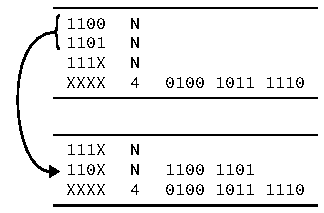
\includegraphics{figures/downcheck_resolve_example_2}
  \end{figure}
  
  We repeat the above process until either no entries are covered (that is $e_m$ does not cover any $e_c$) and a valid merge is produced; or it is not possible to modify the merge to avoid covering a lower entry and the merge must be abandoned.
  In our example, the new merge candidate results in an entry \mytt{110X} being inserted between the bottom two entries.
  As this new entry does not cover any other entries in the table the algorithm terminates.
  
  In our example there were two bits in $e_m$, \mytt{11\underline{XX}}. which could be converted to avoid intersection with $e_c$.
  This is not always the case; \textit{todo...}

  \section{Results}

  \subsection{Compression}

\begin{figure*}
  \centering
  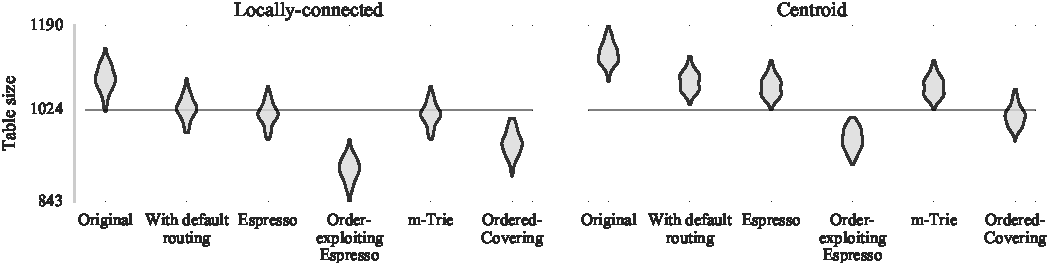
\includegraphics{experiments/results_esp_and_oc}
  \caption{Compression performance of all the routing table minimization schemes for both benchmarks.
           Ordered-Covering minimizes all of the tables in the locally-connected benchmark, and
           \SI{48.6}{\percent} of the tables in the centroid benchmark, to $\le 1024$ entries.
           }
  \label{fig:results/final}
\end{figure*}

  \figurename~\ref{fig:results/final} shows the performance of Ordered-Covering, running on SpiNNaker, when used to minimize the benchmark routing tables.
  While OC does not manage to minimize all of the tables in the centroid benchmark to fewer than 1024 entries it is able to reduce \SI{48.6}{\percent} of the tables to this size.
  This roughly halves the number of tables which would otherwise need to be minimized off-chip.
  OC reduces all of the tables in the locally-connected benchmark to fit in the router TCAM.


  \subsection{Memory usage}

% Gaussian: 18376 bytes of which 13668 bytes is the table
% Centroid: 19152 bytes of which 14328 bytes is the table

  On-chip routing table minimization is required to work with very small amounts of working memory.
  In order-exploiting minimization this small amount of memory must be used to store the whole routing table -- e.g., \SI{24}{\kibi\byte} for a 2048-entry table -- and any additional structures.
  Consequently, those additional structures must be memory efficient.
  After the routing table, the aliases table (which annotates routing table entries with the keys they are expected to match) is the most expensive structure in Ordered-Covering.
  Other structures, such as sets of entries being considered as merge candidates can be implemented using bit-vectors and consume very little memory.

  Each merge of $n$ entries performed by Ordered-Covering reduces the size of the routing table by $n-1$ entries (reducing the memory required to represent the table by $3(n-1)$~words) and adds a new entry into the aliases table.
  In our implementation of the aliases table, which uses AA-trees and linked-lists of fixed-size blocks, a merge of $n$ entries will increase the memory required by the aliases table by $2(n + 1) + 4$~words.
  Consequently, the total memory cost of a merge of $n$ entries is $2(n + 1) + 4 - 3(n - 1)$~words.
  If the space saved by minimizing the routing table were reclaimed (by using a bucket allocator, for example) then any merge of more than ten entries would reduce the memory required to represent the routing and the aliases tables.

  Our implementation of Ordered-Covering does not reclaim the memory saved by reducing the size of a routing table, meaning that the routing table remains a constant size while the aliases table grows with every merge.
  The peak heap usage of our minimizer when running on SpiNNaker was \SI{17.9}{\kibi\byte} for the locally-connected benchmark (of which \SI{13.3}{\kibi\byte} was used to represent the routing table) and \SI{18.7}{\kibi\byte} for the centroid model (\SI{14.0}{\kibi\byte} for the routing table).
  Ordered-Covering is thus able to achieve good levels of table compression for very little memory cost above that required to represent the routing table.

  \subsection{Timing}

  \begin{itemize}
    \item Cursory note about parallelism
    \item Present load and minimize times for benchmarks, for full minimization and sufficient minimization
  \end{itemize}

% \subsection{Hedging}
    
% Each SpiNNaker chip has 18 processor cores and one routing table enabling parallel table minimisation approaches.
% It is possible to execute several table minimisation algorithms simultaneously, terminating as soon as any algorithm produces a table which fits.
% This approach may be valuable in cases where default routing is sufficient since these routes are very cheap to compute.

  \section{Conclusion}

  \begin{itemize}
    \item Routing table minimization a problem for SpiNNaker
    \item Due to small table size, multicast and restricted DTCM existing solutions are insufficient
    \item We introduced Ordered Covering; a memory-efficient order-exploiting routing table minimizer
    \item HEADLINE RESULTS
    \item Future worK:
      \begin{itemize}
        \item Alternative ways of selecting merge candidates may improve performance
        \item Different heuristics for what makes a good merge?
      \end{itemize}
  \end{itemize}

  \section*{Acknowledgements}

  The authors would like to thank James Knight for his helpful feedback on drafts of this paper.

\printbibliography
\end{document}
